\documentclass[aspectratio=169]{beamer}
% \usepackage{enumitem}
\usepackage[utf8]{inputenc}
\usepackage{amsmath, amssymb, amsthm}
\usepackage{algorithm2e}
\usepackage{tikz}
\usepackage{amsmath, amsthm, amssymb}
\usepackage{pgfplots}
\newcommand{\hs}[1]{\hspace*{#1cm}}
\newcommand{\vs}[1]{\vspace*{#1cm}}

\title{Adversarial Uncertainty Quantification in Physics-Informed Neural Networks}
\author{Yibo Yang, Paris Perdikaris}
\institute{University of Pennsylvania}
\date{26.05.2023}

\begin{document}

\maketitle

\section{Introduction}

\begin{frame}{The model: UQPINN}
\begin{minipage}{0.6\textwidth}
{\huge UQPINN = GAN + PINN}
\end{minipage}\hfill
\begin{minipage}{0.4\textwidth}
\begin{enumerate}
    \item \textbf{UQPINN} : Uncertainty Quantification Physics-Informed Neural Network
    \item \textbf{GAN} : Generative Adversarial Network
    \item \textbf{PINN} : Physics-Informed Neural Network
\end{enumerate}
\end{minipage}
\end{frame}

\begin{frame}{Novalty}
"we will develop a flexible \textcolor{orange}{variational inference} framework 
that will allow us to train such models directly from \textcolor{orange}{noisy input/output data}, 
and predict outcomes of non-linear dynamical systems that are partially \textcolor{orange}{observed}
with quantified \textcolor{orange}{uncertainty}"
\hs{1}
\begin{flushright}
    \textit{-- Yibo Yang, Paris Perdikaris}
\end{flushright}
\hs{2}

\uncover<2->{
    \centering
    Using adversarial approach to handle randomness in observations.  
}

\end{frame}

\begin{frame}{GAN}

\begin{minipage}{0.5\textwidth}
    \begin{tikzpicture}[]
        \only<1,4-5>{
            \draw[fill=brown] (0.5, 1) -- (2, 1.5) -- (2, 2.5) -- (0.5, 3) -- cycle;
            \draw[->] (2, 2) .. controls (2.5, 2) and (3, 2) .. (3, 3);
            \draw[->] (0, 2) -- (0.5, 2);
            \draw[] node at (-0.7, 2) {$z\sim p(z)$};
            \draw[] node at (2.5, 1.5) {$p_\theta(x)$};
            \draw[] node at (1, 2) {$f_\theta$};
            \draw[] node at (1.2, 0.7) {generator};
        }
        \only<1-3>{
            \draw[fill=cyan] (3, 2.5) -- (4.5, 2) -- (4.5, 4) -- (3, 3.5) -- cycle;
            \draw[->] (2, 4) .. controls (2.5, 4) and (3, 4) .. (3, 3);
            \draw[->] (4.5, 3) -- (5, 3);
            \draw[] node at (1.7, 4) {$q(x)$};
            \draw[] node at (5.2, 3) {$\rho$};
            \draw[] node at (3.5, 3) {$T_\psi$};
            \draw[] node at (3.9,1.8) {discriminator};
        }
        % \draw[step=0.5, black, thin] (0,0) grid (5, 5); 
        % \foreach \i in {0,0.5,...,5.0} {
		%     \draw [very thin, gray] node [below] at (\i,0) {$\i$};
        %     \draw [very thin, gray] node [left] at (0,\i) {$\i$};
        % }
    \end{tikzpicture}
\end{minipage}\hfill
\begin{minipage}{0.5\textwidth}
\only<1>{
    \begin{align*}
        & \underset{\psi}{max}~\mathcal L_{\mathcal D}(\psi)
        \\
        & \underset{\theta, \phi}{min}~\mathcal L_{\mathcal G}(\theta, \phi) + \beta~\mathcal L_{PDE} (\theta)
    \end{align*}
}
\only<2-3>{
    \begin{align*}
        \underset{\psi}{argmin}&\frac{\rho(y=+1|x,t,u)}{\rho(y=-1|x,t,u)}
        \\
        p_\theta(x,t,u) &= \rho(x,t,u|y=+1)
        \\
        q(x,t,u) &= \rho(x,t,u|y=-1)
    \end{align*}
}
\only<3>{

    $$T_\psi \approx \rho(y=+1|x,t,u)$$
  
    \begin{align*}
        \mathcal L_D(\psi) &= \mathbb E_{q(x,t)p(z)}[log ~\sigma(T_\psi(x,t,f_\theta))] 
        \\
        &+\mathbb E_{q(x,t,u)}[log(1-\sigma(T_\psi))]
    \end{align*}
}
\only<4-5>{
    \begin{align*}
        \underset{\theta}{argmax}~\mathbb{KL}\left[
        p_\theta(x,t,u)
        \Vert
        q(x,t,u)\right]
    \end{align*}
}
\only<5>{
    \begin{align*}
        \mathcal L_G(\theta,\psi) &= \mathbb E_{q(x,t)p(z)}
[T_\psi(x,t,f_\theta(x,t,z))
\\
&+(1-\lambda )log(q_\phi(z|x,t,f_\theta(x,t,z)))]
    \end{align*}
}
\end{minipage}

\end{frame}

\section{Experiment}

\begin{frame}{Experiment Setup}
\begin{tabular}{p{0.2\textwidth}p{0.4\textwidth}p{0.4\textwidth}}
    &{\Large Author's Experiment Setup} & \only<2->{\Large My Experiment Setup}\\[0.5cm]

    \textbf{GPU} & NVIDIA Tesla P100(16GB) & \only<2->{MX450(2GB)}\\[0.2cm]
    
    \textbf{DL framework} & Tensorflow v1.10 & \only<2->{Pytorch v1.9.0}\\[0.2cm]
   
    \textbf{Formula} & \begin{enumerate}
        \item pedagogical ODE
        \item Burgers' equation
        \item Darcy flow
    \end{enumerate} & \only<2->{\begin{enumerate}
        \item pedagogical ODE
        \item Burgers' equation
        \item Darcy flow
    \end{enumerate}}\\
    
    \textbf{Model} & UQPINN & \only<2->{\begin{enumerate}
        \item UQPINN
        \item PINN
    \end{enumerate}}\\
\end{tabular}

\only<3>{    
\centering
    parameters are set to be the same as the author's
}
\end{frame}

\begin{frame}{pedagogical ODE}
$$
\begin{aligned}
\frac{\partial^2 u}{\partial x^2} &- u^2 \frac{\partial u}{\partial x}  f(x) & x&\in[-1,1]
\\
f(x) &= -\pi^2 sin(\pi x) - \pi cos(\pi x)sin(\pi x)^2
\\
u(x) & \sim \mathcal N(sin(\pi), noise)& x&=\{-1,1\}
\end{aligned}
$$
\end{frame}

\begin{frame}{}
    \begin{minipage}[t]{0.5\textwidth}
        \resizebox{\textwidth}{!}{
            % This file was created with tikzplotlib v0.10.1.
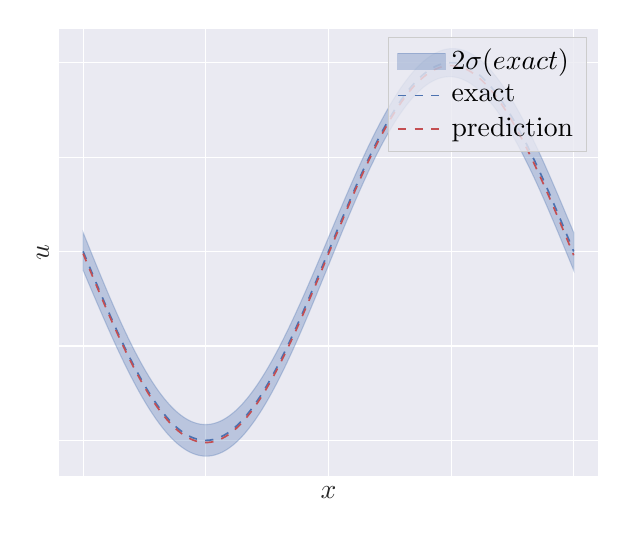
\begin{tikzpicture}

\definecolor{darkslategray38}{RGB}{38,38,38}
\definecolor{indianred1967882}{RGB}{196,78,82}
\definecolor{lavender234234242}{RGB}{234,234,242}
\definecolor{lightgray204}{RGB}{204,204,204}
\definecolor{steelblue76114176}{RGB}{76,114,176}

\begin{axis}[
axis background/.style={fill=lavender234234242},
axis line style={white},
legend cell align={left},
legend style={
  fill opacity=0.8,
  draw opacity=1,
  text opacity=1,
  draw=lightgray204,
  fill=lavender234234242
},
tick align=outside,
x grid style={white},
xlabel=\textcolor{darkslategray38}{\(\displaystyle x\)},
xmajorgrids,
xmajorticks=false,
xmin=-1.1, xmax=1.1,
xtick style={color=darkslategray38},
y grid style={white},
ylabel=\textcolor{darkslategray38}{\(\displaystyle u\)},
ymajorgrids,
ymajorticks=false,
ymin=-1.1910645845124, ymax=1.18239851825652,
ytick style={color=darkslategray38}
]
\path [draw=steelblue76114176, fill=steelblue76114176, opacity=0.3]
(axis cs:-1,0.101009720605508)
--(axis cs:-1,-0.0989959694967012)
--(axis cs:-0.990000009536743,-0.129635291551538)
--(axis cs:-0.980000019073486,-0.160246870075834)
--(axis cs:-0.970000028610229,-0.190801614533027)
--(axis cs:-0.959999978542328,-0.221270437409595)
--(axis cs:-0.949999988079071,-0.251624278952372)
--(axis cs:-0.939999997615814,-0.281834132494592)
--(axis cs:-0.930000007152557,-0.311871070325639)
--(axis cs:-0.920000016689301,-0.34170627005237)
--(axis cs:-0.910000026226044,-0.371311041393941)
--(axis cs:-0.900000035762787,-0.40065685334706)
--(axis cs:-0.89000004529953,-0.429715361654362)
--(axis cs:-0.879999995231628,-0.458458436505498)
--(axis cs:-0.870000004768372,-0.486858190398253)
--(axis cs:-0.860000014305115,-0.51488700608578)
--(axis cs:-0.850000023841858,-0.542517564535537)
--(axis cs:-0.839999973773956,-0.569722872825956)
--(axis cs:-0.829999983310699,-0.596476291907914)
--(axis cs:-0.819999992847443,-0.622751564159932)
--(axis cs:-0.810000002384186,-0.648522840668381)
--(axis cs:-0.799999952316284,-0.673764708166985)
--(axis cs:-0.789999961853027,-0.698452215573288)
--(axis cs:-0.779999971389771,-0.722560900063638)
--(axis cs:-0.769999980926514,-0.746066812632394)
--(axis cs:-0.759999990463257,-0.768946543085552)
--(axis cs:-0.75,-0.79117724442365)
--(axis cs:-0.740000009536743,-0.812736656573699)
--(axis cs:-0.730000019073486,-0.83360312943482)
--(axis cs:-0.719999969005585,-0.853755645207348)
--(axis cs:-0.709999978542328,-0.873173839980194)
--(axis cs:-0.699999988079071,-0.891838024556286)
--(axis cs:-0.689999997615814,-0.909729204500901)
--(axis cs:-0.680000007152557,-0.926829099402509)
--(axis cs:-0.670000016689301,-0.943120161340491)
--(axis cs:-0.660000026226044,-0.958585592558538)
--(axis cs:-0.650000035762787,-0.973209362346858)
--(axis cs:-0.639999985694885,-0.986976223140243)
--(axis cs:-0.629999995231628,-0.99987172584274)
--(axis cs:-0.620000004768372,-1.01188223439291)
--(axis cs:-0.610000014305115,-1.02299493958661)
--(axis cs:-0.600000023841858,-1.03319787217648)
--(axis cs:-0.590000033378601,-1.04247991526947)
--(axis cs:-0.580000042915344,-1.05083081604483)
--(axis cs:-0.570000052452087,-1.05824119681593)
--(axis cs:-0.560000002384186,-1.06470256545946)
--(axis cs:-0.550000011920929,-1.07020732523482)
--(axis cs:-0.540000021457672,-1.07474878401575)
--(axis cs:-0.530000030994415,-1.07832116295383)
--(axis cs:-0.519999980926514,-1.08091960459154)
--(axis cs:-0.509999990463257,-1.08254018043872)
--(axis cs:-0.499999970197678,-1.0831798980229)
--(axis cs:-0.489999979734421,-1.0828367074189)
--(axis cs:-0.479999989271164,-1.08150950725829)
--(axis cs:-0.469999969005585,-1.07919815021363)
--(axis cs:-0.459999978542328,-1.07590344794594)
--(axis cs:-0.449999988079071,-1.07162717549791)
--(axis cs:-0.439999997615814,-1.06637207510814)
--(axis cs:-0.430000007152557,-1.06014185941536)
--(axis cs:-0.419999986886978,-1.05294121401435)
--(axis cs:-0.409999996423721,-1.04477579931918)
--(axis cs:-0.400000005960464,-1.03565225168268)
--(axis cs:-0.389999985694885,-1.02557818371558)
--(axis cs:-0.379999995231628,-1.01456218374358)
--(axis cs:-0.370000004768372,-1.00261381433634)
--(axis cs:-0.360000014305115,-0.989743609838977)
--(axis cs:-0.350000023841858,-0.975963072834616)
--(axis cs:-0.340000003576279,-0.961284669465321)
--(axis cs:-0.330000013113022,-0.945721823539205)
--(axis cs:-0.320000022649765,-0.929288909353079)
--(axis cs:-0.310000002384186,-0.912001243163167)
--(axis cs:-0.300000011920929,-0.893875073240893)
--(axis cs:-0.290000021457672,-0.874927568456701)
--(axis cs:-0.280000001192093,-0.855176805342118)
--(axis cs:-0.270000010728836,-0.834641753588838)
--(axis cs:-0.259999990463257,-0.813342259953203)
--(axis cs:-0.25,-0.791299030545166)
--(axis cs:-0.239999994635582,-0.768533611492213)
--(axis cs:-0.230000004172325,-0.745068367980766)
--(axis cs:-0.219999998807907,-0.720926461690028)
--(axis cs:-0.21000000834465,-0.696131826645741)
--(axis cs:-0.200000002980232,-0.670709143533873)
--(axis cs:-0.189999997615814,-0.644683812526327)
--(axis cs:-0.180000007152557,-0.618081924682422)
--(axis cs:-0.170000001788139,-0.590930232000692)
--(axis cs:-0.159999996423721,-0.563256116205466)
--(axis cs:-0.150000005960464,-0.535087556361381)
--(axis cs:-0.140000000596046,-0.506453095416507)
--(axis cs:-0.13000001013279,-0.477381805780815)
--(axis cs:-0.119999997317791,-0.447903254051335)
--(axis cs:-0.109999999403954,-0.418047464998505)
--(axis cs:-0.0999999940395355,-0.387844884929768)
--(axis cs:-0.0899999961256981,-0.357326344546608)
--(axis cs:-0.0799999982118607,-0.326523021409912)
--(axis cs:-0.0700000002980232,-0.295466402125845)
--(axis cs:-0.0599999986588955,-0.264188244360567)
--(axis cs:-0.0499999970197678,-0.232720538787086)
--(axis cs:-0.0399999991059303,-0.201095471061644)
--(axis cs:-0.0299999993294477,-0.169345383920235)
--(axis cs:-0.0199999995529652,-0.13750273947856)
--(axis cs:-0.00999999884516001,-0.105600081810874)
--(axis cs:8.94069651646845e-10,-0.0736699998751082)
--(axis cs:0.0100000007078052,-0.0417450908434616)
--(axis cs:0.0200000014156103,-0.00985792388947097)
--(axis cs:0.0300000011920929,0.0219589955254169)
--(axis cs:0.0399999991059303,0.0536732608304251)
--(axis cs:0.0500000007450581,0.0852525989611101)
--(axis cs:0.0599999986588955,0.116664904390809)
--(axis cs:0.0700000002980232,0.147878272562741)
--(axis cs:0.0799999982118607,0.178861032713207)
--(axis cs:0.0899999961256981,0.209581780081169)
--(axis cs:0.100000001490116,0.240009407503698)
--(axis cs:0.109999999403954,0.27011313640021)
--(axis cs:0.119999997317791,0.299862547151192)
--(axis cs:0.129999995231628,0.329227608879201)
--(axis cs:0.140000000596046,0.358178708641321)
--(axis cs:0.149999991059303,0.386686680043073)
--(axis cs:0.159999996423721,0.414722831284007)
--(axis cs:0.170000001788139,0.442258972644834)
--(axis cs:0.179999992251396,0.469267443425252)
--(axis cs:0.189999997615814,0.495721138340249)
--(axis cs:0.200000002980232,0.521593533381183)
--(axis cs:0.21000000834465,0.546858711145863)
--(axis cs:0.219999998807907,0.57149138563968)
--(axis cs:0.230000004172325,0.595466926547319)
--(axis cs:0.240000009536743,0.618761382971878)
--(axis cs:0.25,0.641351506635402)
--(axis cs:0.259999990463257,0.66321477453182)
--(axis cs:0.270000010728836,0.684329411020236)
--(axis cs:0.280000001192093,0.704674409343374)
--(axis cs:0.28999999165535,0.724229552552814)
--(axis cs:0.300000011920929,0.74297543381952)
--(axis cs:0.310000002384186,0.760893476104967)
--(axis cs:0.319999992847443,0.77796595116513)
--(axis cs:0.330000013113022,0.794175997856559)
--(axis cs:0.340000003576279,0.809507639710848)
--(axis cs:0.349999994039536,0.823945801741052)
--(axis cs:0.360000014305115,0.837476326440976)
--(axis cs:0.370000004768372,0.850085988935884)
--(axis cs:0.380000025033951,0.861762511240991)
--(axis cs:0.390000015497208,0.872494575582242)
--(axis cs:0.400000005960464,0.882271836732329)
--(axis cs:0.410000026226044,0.891084933313753)
--(axis cs:0.420000016689301,0.898925498019945)
--(axis cs:0.430000007152557,0.905786166705262)
--(axis cs:0.439999997615814,0.911660586294904)
--(axis cs:0.449999988079071,0.916543421466637)
--(axis cs:0.46000000834465,0.920430360057729)
--(axis cs:0.469999998807907,0.92331811715259)
--(axis cs:0.479999989271164,0.9252044378095)
--(axis cs:0.490000009536743,0.926088098388371)
--(axis cs:0.5,0.925968906445831)
--(axis cs:0.509999990463257,0.924847699168986)
--(axis cs:0.519999980926514,0.922726340325067)
--(axis cs:0.529999971389771,0.91960771571071)
--(axis cs:0.539999961853027,0.915495727091835)
--(axis cs:0.549999952316284,0.910395284632934)
--(axis cs:0.560000002384186,0.904312297822966)
--(axis cs:0.569999992847443,0.897253664913845)
--(axis cs:0.579999983310699,0.889227260896655)
--(axis cs:0.589999973773956,0.880241924050077)
--(axis cs:0.600000023841858,0.870307441104816)
--(axis cs:0.610000014305115,0.859434531077167)
--(axis cs:0.620000004768372,0.847634827833758)
--(axis cs:0.629999995231628,0.834920861458085)
--(axis cs:0.64000004529953,0.821306038497346)
--(axis cs:0.650000035762787,0.806804621175223)
--(axis cs:0.660000026226044,0.791431705662388)
--(axis cs:0.670000016689301,0.775203199501659)
--(axis cs:0.680000007152557,0.758135798288529)
--(axis cs:0.689999997615814,0.740246961710355)
--(axis cs:0.699999988079071,0.721554889048627)
--(axis cs:0.709999978542328,0.70207849424836)
--(axis cs:0.720000028610229,0.681837380656918)
--(axis cs:0.730000019073486,0.660851815531214)
--(axis cs:0.740000009536743,0.639142704407622)
--(axis cs:0.75,0.616731565422865)
--(axis cs:0.759999990463257,0.5936405036669)
--(axis cs:0.769999980926514,0.569892185640516)
--(axis cs:0.779999971389771,0.545509813881088)
--(axis cs:0.789999961853027,0.520517101809988)
--(axis cs:0.800000011920929,0.494938248844667)
--(axis cs:0.810000002384186,0.468797915807632)
--(axis cs:0.819999992847443,0.442121200653716)
--(axis cs:0.829999983310699,0.414933614526298)
--(axis cs:0.839999973773956,0.387261058142833)
--(axis cs:0.849999964237213,0.35912979850025)
--(axis cs:0.85999995470047,0.330566445881817)
--(axis cs:0.869999945163727,0.301597931138932)
--(axis cs:0.879999995231628,0.272251483214377)
--(axis cs:0.889999985694885,0.242554606867667)
--(axis cs:0.899999976158142,0.212535060558646)
--(axis cs:0.909999966621399,0.182220834442181)
--(axis cs:0.920000016689301,0.151640128424986)
--(axis cs:0.930000007152557,0.120821330234965)
--(axis cs:0.939999997615814,0.0897929934542626)
--(axis cs:0.949999988079071,0.0585838154691073)
--(axis cs:0.959999978542328,0.0272226152926647)
--(axis cs:0.970000028610229,-0.00426168877876204)
--(axis cs:0.980000019073486,-0.0358401017108175)
--(axis cs:0.990000009536743,-0.0674835745063249)
--(axis cs:1,-0.0991630272330932)
--(axis cs:1,0.10064283509553)
--(axis cs:1,0.10064283509553)
--(axis cs:0.990000009536743,0.131788460683482)
--(axis cs:0.980000019073486,0.162906488484171)
--(axis cs:0.970000028610229,0.193964051810253)
--(axis cs:0.959999978542328,0.224928377016329)
--(axis cs:0.949999988079071,0.255766821969704)
--(axis cs:0.939999997615814,0.286446914575803)
--(axis cs:0.930000007152557,0.316936391270315)
--(axis cs:0.920000016689301,0.347203235383848)
--(axis cs:0.909999966621399,0.377215715279379)
--(axis cs:0.899999976158142,0.40694242215831)
--(axis cs:0.889999985694885,0.436352307427434)
--(axis cs:0.879999995231628,0.465414719516962)
--(axis cs:0.869999945163727,0.494099440038692)
--(axis cs:0.85999995470047,0.52237671917399)
--(axis cs:0.849999964237213,0.550217310183038)
--(axis cs:0.839999973773956,0.577592502930294)
--(axis cs:0.829999983310699,0.604474156325883)
--(axis cs:0.819999992847443,0.630834729589)
--(axis cs:0.810000002384186,0.656647312247006)
--(axis cs:0.800000011920929,0.68188565279285)
--(axis cs:0.789999961853027,0.706524185933461)
--(axis cs:0.779999971389771,0.730538058372728)
--(axis cs:0.769999980926514,0.75390315308444)
--(axis cs:0.759999990463257,0.77659611204284)
--(axis cs:0.75,0.79859435739106)
--(axis cs:0.740000009536743,0.819876111040377)
--(axis cs:0.730000019073486,0.840420412705784)
--(axis cs:0.720000028610229,0.860207136395485)
--(axis cs:0.709999978542328,0.879217005383455)
--(axis cs:0.699999988079071,0.897431605704861)
--(axis cs:0.689999997615814,0.914833398223818)
--(axis cs:0.680000007152557,0.931405729331403)
--(axis cs:0.670000016689301,0.947132840338993)
--(axis cs:0.660000026226044,0.961999875637719)
--(axis cs:0.650000035762787,0.975992889699028)
--(axis cs:0.64000004529953,0.989098852994075)
--(axis cs:0.629999995231628,1.00130565691083)
--(axis cs:0.620000004768372,1.01260211774748)
--(axis cs:0.610000014305115,1.02297797985908)
--(axis cs:0.600000023841858,1.03242391803117)
--(axis cs:0.589999973773956,1.04093153915034)
--(axis cs:0.579999983310699,1.04849338323579)
--(axis cs:0.569999992847443,1.05510292389064)
--(axis cs:0.560000002384186,1.06075456822419)
--(axis cs:0.549999952316284,1.06544365628949)
--(axis cs:0.539999961853027,1.0691664600726)
--(axis cs:0.529999971389771,1.07192018206222)
--(axis cs:0.519999980926514,1.07370295342034)
--(axis cs:0.509999990463257,1.07451383176702)
--(axis cs:0.5,1.07435279858469)
--(axis cs:0.490000009536743,1.07322075624063)
--(axis cs:0.479999989271164,1.0711195246196)
--(axis cs:0.469999998807907,1.06805183735277)
--(axis cs:0.46000000834465,1.06402133762379)
--(axis cs:0.449999988079071,1.05903257352854)
--(axis cs:0.439999997615814,1.05309099296129)
--(axis cs:0.430000007152557,1.04620293799683)
--(axis cs:0.420000016689301,1.03837563873645)
--(axis cs:0.410000026226044,1.02961720658379)
--(axis cs:0.400000005960464,1.0199366269161)
--(axis cs:0.390000015497208,1.0093437511164)
--(axis cs:0.380000025033951,0.997849287932852)
--(axis cs:0.370000004768372,0.985464794132594)
--(axis cs:0.360000014305115,0.972202664419469)
--(axis cs:0.349999994039536,0.958076120587091)
--(axis cs:0.340000003576279,0.943099199881578)
--(axis cs:0.330000013113022,0.927286742551328)
--(axis cs:0.319999992847443,0.910654378564679)
--(axis cs:0.310000002384186,0.89321851347997)
--(axis cs:0.300000011920929,0.874996313456492)
--(axis cs:0.28999999165535,0.856005689398928)
--(axis cs:0.280000001192093,0.836265280232127)
--(axis cs:0.270000010728836,0.815794435307481)
--(axis cs:0.259999990463257,0.794613195946577)
--(axis cs:0.25,0.772742276132341)
--(axis cs:0.240000009536743,0.750203042362375)
--(axis cs:0.230000004172325,0.727017492683737)
--(axis cs:0.219999998807907,0.703208234932857)
--(axis cs:0.21000000834465,0.678798464208736)
--(axis cs:0.200000002980232,0.653811939611894)
--(axis cs:0.189999997615814,0.628272960285772)
--(axis cs:0.179999992251396,0.602206340801365)
--(axis cs:0.170000001788139,0.57563738592979)
--(axis cs:0.159999996423721,0.548591864851199)
--(axis cs:0.149999991059303,0.521095984851894)
--(axis cs:0.140000000596046,0.493176364564714)
--(axis cs:0.129999995231628,0.464860006810582)
--(axis cs:0.119999997317791,0.436174271101614)
--(axis cs:0.109999999403954,0.407146845868251)
--(axis cs:0.100000001490116,0.377805720474465)
--(axis cs:0.0899999961256981,0.348179157086207)
--(axis cs:0.0799999982118607,0.318295662458782)
--(axis cs:0.0700000002980232,0.288183959708766)
--(axis cs:0.0599999986588955,0.257872960135383)
--(axis cs:0.0500000007450581,0.227391735154868)
--(axis cs:0.0399999991059303,0.196769488409256)
--(axis cs:0.0300000011920929,0.166035528108213)
--(axis cs:0.0200000014156103,0.13521923965902)
--(axis cs:0.0100000007078052,0.104350058635538)
--(axis cs:8.94069651646845e-10,0.0734574441320207)
--(axis cs:-0.00999999884516001,0.0425708525420204)
--(axis cs:-0.0199999995529652,0.0117197117963772)
--(axis cs:-0.0299999993294477,-0.0190666039125227)
--(axis cs:-0.0399999991059303,-0.0497587989003058)
--(axis cs:-0.0499999970197678,-0.0803276802417129)
--(axis cs:-0.0599999986588955,-0.110744181498867)
--(axis cs:-0.0700000002980232,-0.140979385930339)
--(axis cs:-0.0799999982118607,-0.171004549192669)
--(axis cs:-0.0899999961256981,-0.200791121553792)
--(axis cs:-0.0999999940395355,-0.23031076964538)
--(axis cs:-0.109999999403954,-0.259535397788062)
--(axis cs:-0.119999997317791,-0.288437168929928)
--(axis cs:-0.13000001013279,-0.31698852524424)
--(axis cs:-0.140000000596046,-0.345162208436948)
--(axis cs:-0.150000005960464,-0.372931279818115)
--(axis cs:-0.159999996423721,-0.40026914019379)
--(axis cs:-0.170000001788139,-0.427149549635892)
--(axis cs:-0.180000007152557,-0.453546647187489)
--(axis cs:-0.189999997615814,-0.479434970559191)
--(axis cs:-0.200000002980232,-0.50478947586941)
--(axis cs:-0.21000000834465,-0.529585557476872)
--(axis cs:-0.219999998807907,-0.553799067948164)
--(axis cs:-0.230000004172325,-0.577406338196208)
--(axis cs:-0.239999994635582,-0.600384197817711)
--(axis cs:-0.25,-0.622709995648739)
--(axis cs:-0.259999990463257,-0.644361620548)
--(axis cs:-0.270000010728836,-0.665317522407273)
--(axis cs:-0.280000001192093,-0.685556733377864)
--(axis cs:-0.290000021457672,-0.705058889291379)
--(axis cs:-0.300000011920929,-0.723804251242488)
--(axis cs:-0.310000002384186,-0.74177372729111)
--(axis cs:-0.320000022649765,-0.75894889423169)
--(axis cs:-0.330000013113022,-0.775312019368183)
--(axis cs:-0.340000003576279,-0.790846082225184)
--(axis cs:-0.350000023841858,-0.805534796118555)
--(axis cs:-0.360000014305115,-0.819362629502869)
--(axis cs:-0.370000004768372,-0.832314827008386)
--(axis cs:-0.379999995231628,-0.844377430076849)
--(axis cs:-0.389999985694885,-0.855537297103454)
--(axis cs:-0.400000005960464,-0.865782122991723)
--(axis cs:-0.409999996423721,-0.875100458028786)
--(axis cs:-0.419999986886978,-0.883481725990624)
--(axis cs:-0.430000007152557,-0.890916241390103)
--(axis cs:-0.439999997615814,-0.897395225785072)
--(axis cs:-0.449999988079071,-0.90291082306916)
--(axis cs:-0.459999978542328,-0.907456113674235)
--(axis cs:-0.469999969005585,-0.911025127620451)
--(axis cs:-0.479999989271164,-0.913612856357428)
--(axis cs:-0.489999979734421,-0.915215263348053)
--(axis cs:-0.499999970197678,-0.915829293354695)
--(axis cs:-0.509999990463257,-0.915452880395947)
--(axis cs:-0.519999980926514,-0.914084954350413)
--(axis cs:-0.530000030994415,-0.911725446192175)
--(axis cs:-0.540000021457672,-0.908375291850576)
--(axis cs:-0.550000011920929,-0.9040364346944)
--(axis cs:-0.560000002384186,-0.898711826647701)
--(axis cs:-0.570000052452087,-0.892405427950972)
--(axis cs:-0.580000042915344,-0.885122205587354)
--(axis cs:-0.590000033378601,-0.87686813039882)
--(axis cs:-0.600000023841858,-0.867650172921934)
--(axis cs:-0.610000014305115,-0.857476297976666)
--(axis cs:-0.620000004768372,-0.846355458045031)
--(axis cs:-0.629999995231628,-0.834297585478826)
--(axis cs:-0.639999985694885,-0.821313583577652)
--(axis cs:-0.650000035762787,-0.8074153165796)
--(axis cs:-0.660000026226044,-0.792615598607611)
--(axis cs:-0.670000016689301,-0.776928181614526)
--(axis cs:-0.680000007152557,-0.760367742369294)
--(axis cs:-0.689999997615814,-0.742949868525777)
--(axis cs:-0.699999988079071,-0.724691043814041)
--(axis cs:-0.709999978542328,-0.705608632392097)
--(axis cs:-0.719999969005585,-0.685720862393677)
--(axis cs:-0.730000019073486,-0.665046808704975)
--(axis cs:-0.740000009536743,-0.643606375000253)
--(axis cs:-0.75,-0.621420275062975)
--(axis cs:-0.759999990463257,-0.598510013415637)
--(axis cs:-0.769999980926514,-0.574897865277816)
--(axis cs:-0.779999971389771,-0.550606855868151)
--(axis cs:-0.789999961853027,-0.52566073906212)
--(axis cs:-0.799999952316284,-0.500083975413519)
--(axis cs:-0.810000002384186,-0.473901709543695)
--(axis cs:-0.819999992847443,-0.447139746898697)
--(axis cs:-0.829999983310699,-0.419824529870824)
--(axis cs:-0.839999973773956,-0.391983113277517)
--(axis cs:-0.850000023841858,-0.363643139187229)
--(axis cs:-0.860000014305115,-0.334832811079011)
--(axis cs:-0.870000004768372,-0.305580867319873)
--(axis cs:-0.879999995231628,-0.275916553941995)
--(axis cs:-0.89000004529953,-0.245869596700174)
--(axis cs:-0.900000035762787,-0.215470172389024)
--(axis cs:-0.910000026226044,-0.184748879399125)
--(axis cs:-0.920000016689301,-0.153736707491874)
--(axis cs:-0.930000007152557,-0.12246500677404)
--(axis cs:-0.939999997615814,-0.0909654558553347)
--(axis cs:-0.949999988079071,-0.0592700291753882)
--(axis cs:-0.959999978542328,-0.0274109634906891)
--(axis cs:-0.970000028610229,0.00457927648285796)
--(axis cs:-0.980000019073486,0.0366680332699558)
--(axis cs:-0.990000009536743,0.0688224926695994)
--(axis cs:-1,0.101009720605508)
--cycle;
\addlegendimage{area legend, draw=steelblue76114176, fill=steelblue76114176, opacity=0.3}
\addlegendentry{$2\sigma(exact)$}

\addplot [semithick, steelblue76114176, dashed]
table {%
-1 0.00100687555440365
-0.990000009536743 -0.0304063994409693
-0.980000019073486 -0.061789418402939
-0.970000028610229 -0.0931111690250844
-0.959999978542328 -0.124340700450142
-0.949999988079071 -0.15544715406388
-0.939999997615814 -0.186399794174963
-0.930000007152557 -0.21716803854984
-0.920000016689301 -0.247721488772122
-0.910000026226044 -0.278029960396533
-0.900000035762787 -0.308063512868042
-0.89000004529953 -0.337792479177268
-0.879999995231628 -0.367187495223747
-0.870000004768372 -0.396219528859063
-0.860000014305115 -0.424859908582395
-0.850000023841858 -0.453080351861383
-0.839999973773956 -0.480852993051736
-0.829999983310699 -0.508150410889369
-0.819999992847443 -0.534945655529314
-0.810000002384186 -0.561212275106038
-0.799999952316284 -0.586924341790252
-0.789999961853027 -0.612056477317704
-0.779999971389771 -0.636583877965895
-0.769999980926514 -0.660482338955105
-0.759999990463257 -0.683728278250594
-0.75 -0.706298759743312
-0.740000009536743 -0.728171515786976
-0.730000019073486 -0.749324969069897
-0.719999969005585 -0.769738253800513
-0.709999978542328 -0.789391236186145
-0.699999988079071 -0.808264534185164
-0.689999997615814 -0.826339536513339
-0.680000007152557 -0.843598420885902
-0.670000016689301 -0.860024171477508
-0.660000026226044 -0.875600595583074
-0.650000035762787 -0.890312339463229
-0.639999985694885 -0.904144903358947
-0.629999995231628 -0.917084655660783
-0.620000004768372 -0.929118846218971
-0.610000014305115 -0.940235618781637
-0.600000023841858 -0.950424022549207
-0.590000033378601 -0.959674022834146
-0.580000042915344 -0.967976510816091
-0.570000052452087 -0.975323312383452
-0.560000002384186 -0.981707196053578
-0.550000011920929 -0.987121879964612
-0.540000021457672 -0.991562037933164
-0.530000030994415 -0.995023304573005
-0.519999980926514 -0.997502279470974
-0.509999990463257 -0.998996530417333
-0.499999970197678 -0.999504595688799
-0.489999979734421 -0.999025985383475
-0.479999989271164 -0.997561181807859
-0.469999969005585 -0.995111638917039
-0.459999978542328 -0.991679780810087
-0.449999988079071 -0.987268999283534
-0.439999997615814 -0.981883650446608
-0.430000007152557 -0.975529050402732
-0.419999986886978 -0.968211470002488
-0.409999996423721 -0.959938128673986
-0.400000005960464 -0.950717187337203
-0.389999985694885 -0.940557740409518
-0.379999995231628 -0.929469806910216
-0.370000004768372 -0.917464320672363
-0.360000014305115 -0.904553119670923
-0.350000023841858 -0.890748934476585
-0.340000003576279 -0.876065375845252
-0.330000013113022 -0.860516921453694
-0.320000022649765 -0.844118901792385
-0.310000002384186 -0.826887485227139
-0.300000011920929 -0.808839662241691
-0.290000021457672 -0.78999322887404
-0.280000001192093 -0.770366769359991
-0.270000010728836 -0.749979637998056
-0.259999990463257 -0.728851940250602
-0.25 -0.707004513096953
-0.239999994635582 -0.684458904654962
-0.230000004172325 -0.661237353088487
-0.219999998807907 -0.637362764819096
-0.21000000834465 -0.612858692061307
-0.200000002980232 -0.587749309701641
-0.189999997615814 -0.562059391542759
-0.180000007152557 -0.535814285934955
-0.170000001788139 -0.509039890818292
-0.159999996423721 -0.481762628199628
-0.150000005960464 -0.454009418089748
-0.140000000596046 -0.425807651926728
-0.13000001013279 -0.397185165512527
-0.119999997317791 -0.368170211490631
-0.109999999403954 -0.338791431393283
-0.0999999940395355 -0.309077827287574
-0.0899999961256981 -0.2790587330502
-0.0799999982118607 -0.24876378530129
-0.0700000002980232 -0.218222894028092
-0.0599999986588955 -0.187466212929717
-0.0499999970197678 -0.156524109514399
-0.0399999991059303 -0.125427134980975
-0.0299999993294477 -0.0942059939163786
-0.0199999995529652 -0.0628915138410916
-0.00999999884516001 -0.031514614634427
8.94069651646845e-10 -0.00010627787154376
0.0100000007078052 0.0313024838960381
0.0200000014156103 0.0626806578847743
0.0300000011920929 0.0939972618168148
0.0399999991059303 0.125221374619841
0.0500000007450581 0.156322167057989
0.0599999986588955 0.187268932263096
0.0700000002980232 0.218031116135753
0.0799999982118607 0.248578347585995
0.0899999961256981 0.278880468583688
0.100000001490116 0.308907563989082
0.109999999403954 0.33862999113423
0.119999997317791 0.368018409126403
0.129999995231628 0.397043807844891
0.140000000596046 0.425677536603018
0.149999991059303 0.453891332447484
0.159999996423721 0.481657348067603
0.170000001788139 0.508948179287312
0.179999992251396 0.535736892113308
0.189999997615814 0.561997049313011
0.200000002980232 0.587702736496539
0.21000000834465 0.612828587677299
0.219999998807907 0.637349810286269
0.230000004172325 0.661242209615528
0.240000009536743 0.684482212667126
0.25 0.707046891383871
0.259999990463257 0.728913985239198
0.270000010728836 0.750061923163859
0.280000001192093 0.77046984478775
0.28999999165535 0.790117620975871
0.300000011920929 0.808985873638006
0.310000002384186 0.827055994792468
0.319999992847443 0.844310164864904
0.330000013113022 0.860731370203944
0.340000003576279 0.876303419796213
0.349999994039536 0.891010961164072
0.360000014305115 0.904839495430222
0.370000004768372 0.917775391534239
0.380000025033951 0.929805899586922
0.390000015497208 0.940919163349321
0.400000005960464 0.951104231824213
0.410000026226044 0.960351069948773
0.420000016689301 0.968650568378196
0.430000007152557 0.975994552351045
0.439999997615814 0.982375789628097
0.449999988079071 0.98778799749759
0.46000000834465 0.992225848840757
0.469999998807907 0.995684977252681
0.479999989271164 0.998161981214552
0.490000009536743 0.999654427314499
0.5 1.00016085251526
0.509999990463257 0.999680765468003
0.519999980926514 0.998214646872703
0.529999971389771 0.995763948886463
0.539999961853027 0.992331093582219
0.549999952316284 0.987919470461214
0.560000002384186 0.98253343302358
0.569999992847443 0.976178294402241
0.579999983310699 0.968860322066221
0.589999973773956 0.960586731600206
0.600000023841858 0.951365679567994
0.610000014305115 0.941206255468122
0.620000004768372 0.930118472790621
0.629999995231628 0.918113259184457
0.64000004529953 0.90520244574571
0.650000035762787 0.891398755437125
0.660000026226044 0.876715790650053
0.670000016689301 0.861168019920326
0.680000007152557 0.844770763809966
0.689999997615814 0.827540179967087
0.699999988079071 0.809493247376744
0.709999978542328 0.790647749815908
0.720000028610229 0.771022258526202
0.730000019073486 0.750636114118499
0.740000009536743 0.729509407724
0.75 0.707662961406962
0.759999990463257 0.68511830785487
0.769999980926514 0.661897669362478
0.779999971389771 0.638023936126908
0.789999961853027 0.613520643871725
0.800000011920929 0.588411950818758
0.810000002384186 0.562722614027319
0.819999992847443 0.536477965121358
0.829999983310699 0.50970388542609
0.839999973773956 0.482426780536563
0.849999964237213 0.454673554341644
0.85999995470047 0.426471582527904
0.869999945163727 0.397848685588812
0.879999995231628 0.368833101365669
0.889999985694885 0.33945345714755
0.899999976158142 0.309738741358478
0.909999966621399 0.27971827486078
0.920000016689301 0.249421681904417
0.930000007152557 0.21887886075264
0.939999997615814 0.188119954015033
0.949999988079071 0.157175318719406
0.959999978542328 0.126075496154497
0.970000028610229 0.0948511815157453
0.980000019073486 0.0635331933866765
0.990000009536743 0.0321524430885783
1 0.000739903931218498
};
\addlegendentry{exact}
\addplot [semithick, indianred1967882, dashed]
table {%
-1 -0.011030082590878
-0.990000009536743 -0.0423606894910336
-0.980000019073486 -0.0736348778009415
-0.970000028610229 -0.104829184710979
-0.959999978542328 -0.13591867685318
-0.949999988079071 -0.166877582669258
-0.939999997615814 -0.197679534554482
-0.930000007152557 -0.228298351168633
-0.920000016689301 -0.258708029985428
-0.910000026226044 -0.288880527019501
-0.900000035762787 -0.318789154291153
-0.89000004529953 -0.348404794931412
-0.879999995231628 -0.377700716257095
-0.870000004768372 -0.406649321317673
-0.860000014305115 -0.435222446918488
-0.850000023841858 -0.46339026093483
-0.839999973773956 -0.491128087043762
-0.829999983310699 -0.518405675888062
-0.819999992847443 -0.545195996761322
-0.810000002384186 -0.571472108364105
-0.799999952316284 -0.597207605838776
-0.789999961853027 -0.622374594211578
-0.779999971389771 -0.646947920322418
-0.769999980926514 -0.670900881290436
-0.759999990463257 -0.694210231304169
-0.75 -0.716850459575653
-0.740000009536743 -0.738797664642334
-0.730000019073486 -0.76002836227417
-0.719999969005585 -0.780521154403687
-0.709999978542328 -0.800253868103027
-0.699999988079071 -0.819206357002258
-0.689999997615814 -0.837357878684998
-0.680000007152557 -0.854690670967102
-0.670000016689301 -0.871186494827271
-0.660000026226044 -0.886827647686005
-0.650000035762787 -0.901599168777466
-0.639999985694885 -0.915484368801117
-0.629999995231628 -0.928470492362976
-0.620000004768372 -0.940544724464417
-0.610000014305115 -0.951695203781128
-0.600000023841858 -0.961909651756287
-0.590000033378601 -0.971179604530334
-0.580000042915344 -0.97949606180191
-0.570000052452087 -0.986851215362549
-0.560000002384186 -0.993237614631653
-0.550000011920929 -0.998651266098022
-0.540000021457672 -1.00308620929718
-0.530000030994415 -1.00653958320618
-0.519999980926514 -1.00900840759277
-0.509999990463257 -1.01049137115479
-0.499999970197678 -1.01098823547363
-0.489999979734421 -1.01049911975861
-0.479999989271164 -1.00902533531189
-0.469999969005585 -1.00656926631927
-0.459999978542328 -1.00313460826874
-0.449999988079071 -0.998724818229675
-0.439999997615814 -0.993344902992249
-0.430000007152557 -0.987001657485962
-0.419999986886978 -0.979701280593872
-0.409999996423721 -0.971451342105865
-0.400000005960464 -0.962261319160461
-0.389999985694885 -0.952139019966125
-0.379999995231628 -0.94109582901001
-0.370000004768372 -0.92914080619812
-0.360000014305115 -0.91628760099411
-0.350000023841858 -0.902548551559448
-0.340000003576279 -0.887935757637024
-0.330000013113022 -0.872464060783386
-0.320000022649765 -0.856147527694702
-0.310000002384186 -0.839002251625061
-0.300000011920929 -0.821044266223907
-0.290000021457672 -0.802290558815002
-0.280000001192093 -0.782758116722107
-0.270000010728836 -0.762466132640839
-0.259999990463257 -0.741433680057526
-0.25 -0.71968013048172
-0.239999994635582 -0.697226405143738
-0.230000004172325 -0.67409348487854
-0.219999998807907 -0.65030300617218
-0.21000000834465 -0.625878393650055
-0.200000002980232 -0.600842177867889
-0.189999997615814 -0.575218677520752
-0.180000007152557 -0.549032092094421
-0.170000001788139 -0.522308111190796
-0.159999996423721 -0.49507212638855
-0.150000005960464 -0.467351049184799
-0.140000000596046 -0.439171642065048
-0.13000001013279 -0.410561442375183
-0.119999997317791 -0.381548792123795
-0.109999999403954 -0.352162271738052
-0.0999999940395355 -0.322431206703186
-0.0899999961256981 -0.29238498210907
-0.0799999982118607 -0.262053638696671
-0.0700000002980232 -0.231467947363853
-0.0599999986588955 -0.200658410787582
-0.0499999970197678 -0.169656291604042
-0.0399999991059303 -0.138492971658707
-0.0299999993294477 -0.107200115919113
-0.0199999995529652 -0.075809545814991
-0.00999999884516001 -0.0443531647324562
8.94069651646845e-10 -0.012863208539784
0.0100000007078052 0.018628153949976
0.0200000014156103 0.0500887520611286
0.0300000011920929 0.0814865529537201
0.0399999991059303 0.11278934776783
0.0500000007450581 0.143965169787407
0.0599999986588955 0.174982160329819
0.0700000002980232 0.205808877944946
0.0799999982118607 0.236413955688477
0.0899999961256981 0.266766279935837
0.100000001490116 0.29683518409729
0.109999999403954 0.326590359210968
0.119999997317791 0.356001704931259
0.129999995231628 0.385040074586868
0.140000000596046 0.413676261901855
0.149999991059303 0.441881477832794
0.159999996423721 0.46962833404541
0.170000001788139 0.49688908457756
0.179999992251396 0.523637056350708
0.189999997615814 0.549845814704895
0.200000002980232 0.575490176677704
0.21000000834465 0.600544929504395
0.219999998807907 0.624986052513123
0.230000004172325 0.648789465427399
0.240000009536743 0.671932816505432
0.25 0.694393754005432
0.259999990463257 0.716150760650635
0.270000010728836 0.737183034420013
0.280000001192093 0.757470667362213
0.28999999165535 0.776994347572327
0.300000011920929 0.795735538005829
0.310000002384186 0.813676357269287
0.319999992847443 0.830800116062164
0.330000013113022 0.847089529037476
0.340000003576279 0.862530529499054
0.349999994039536 0.877107858657837
0.360000014305115 0.890806615352631
0.370000004768372 0.903614938259125
0.380000025033951 0.915519893169403
0.390000015497208 0.92650979757309
0.400000005960464 0.936574220657349
0.410000026226044 0.945703029632568
0.420000016689301 0.953886866569519
0.430000007152557 0.961117565631866
0.439999997615814 0.967387676239014
0.449999988079071 0.972691357135773
0.46000000834465 0.977022230625153
0.469999998807907 0.980375170707703
0.479999989271164 0.982747197151184
0.490000009536743 0.984134495258331
0.5 0.984535455703735
0.509999990463257 0.983948886394501
0.519999980926514 0.982374548912048
0.529999971389771 0.979813277721405
0.539999961853027 0.976267039775848
0.549999952316284 0.971738636493683
0.560000002384186 0.966231286525726
0.569999992847443 0.959750473499298
0.579999983310699 0.95230233669281
0.589999973773956 0.943892359733582
0.600000023841858 0.93452912569046
0.610000014305115 0.924222409725189
0.620000004768372 0.912981450557709
0.629999995231628 0.900816202163696
0.64000004529953 0.887740969657898
0.650000035762787 0.8737673163414
0.660000026226044 0.858908891677856
0.670000016689301 0.843181788921356
0.680000007152557 0.826600849628448
0.689999997615814 0.809184074401855
0.699999988079071 0.790949940681458
0.709999978542328 0.771915793418884
0.720000028610229 0.752102375030518
0.730000019073486 0.731530249118805
0.740000009536743 0.710219740867615
0.75 0.688194990158081
0.759999990463257 0.665476977825165
0.769999980926514 0.642090976238251
0.779999971389771 0.618060290813446
0.789999961853027 0.593411147594452
0.800000011920929 0.568167924880981
0.810000002384186 0.542356789112091
0.819999992847443 0.516004204750061
0.829999983310699 0.489137589931488
0.839999973773956 0.461783111095428
0.849999964237213 0.4339699447155
0.85999995470047 0.405724138021469
0.869999945163727 0.377074629068375
0.879999995231628 0.34804892539978
0.889999985694885 0.318675726652145
0.899999976158142 0.288981229066849
0.909999966621399 0.258995175361633
0.920000016689301 0.228745132684708
0.930000007152557 0.198258087038994
0.939999997615814 0.167562112212181
0.949999988079071 0.136682704091072
0.959999978542328 0.105647087097168
0.970000028610229 0.0744828507304192
0.980000019073486 0.043213564902544
0.990000009536743 0.0118657667189837
1 -0.0195354819297791
};
\addlegendentry{prediction}
\end{axis}

\end{tikzpicture}

        }
    \end{minipage}\hfill
    \begin{minipage}[t]{0.5\textwidth}
        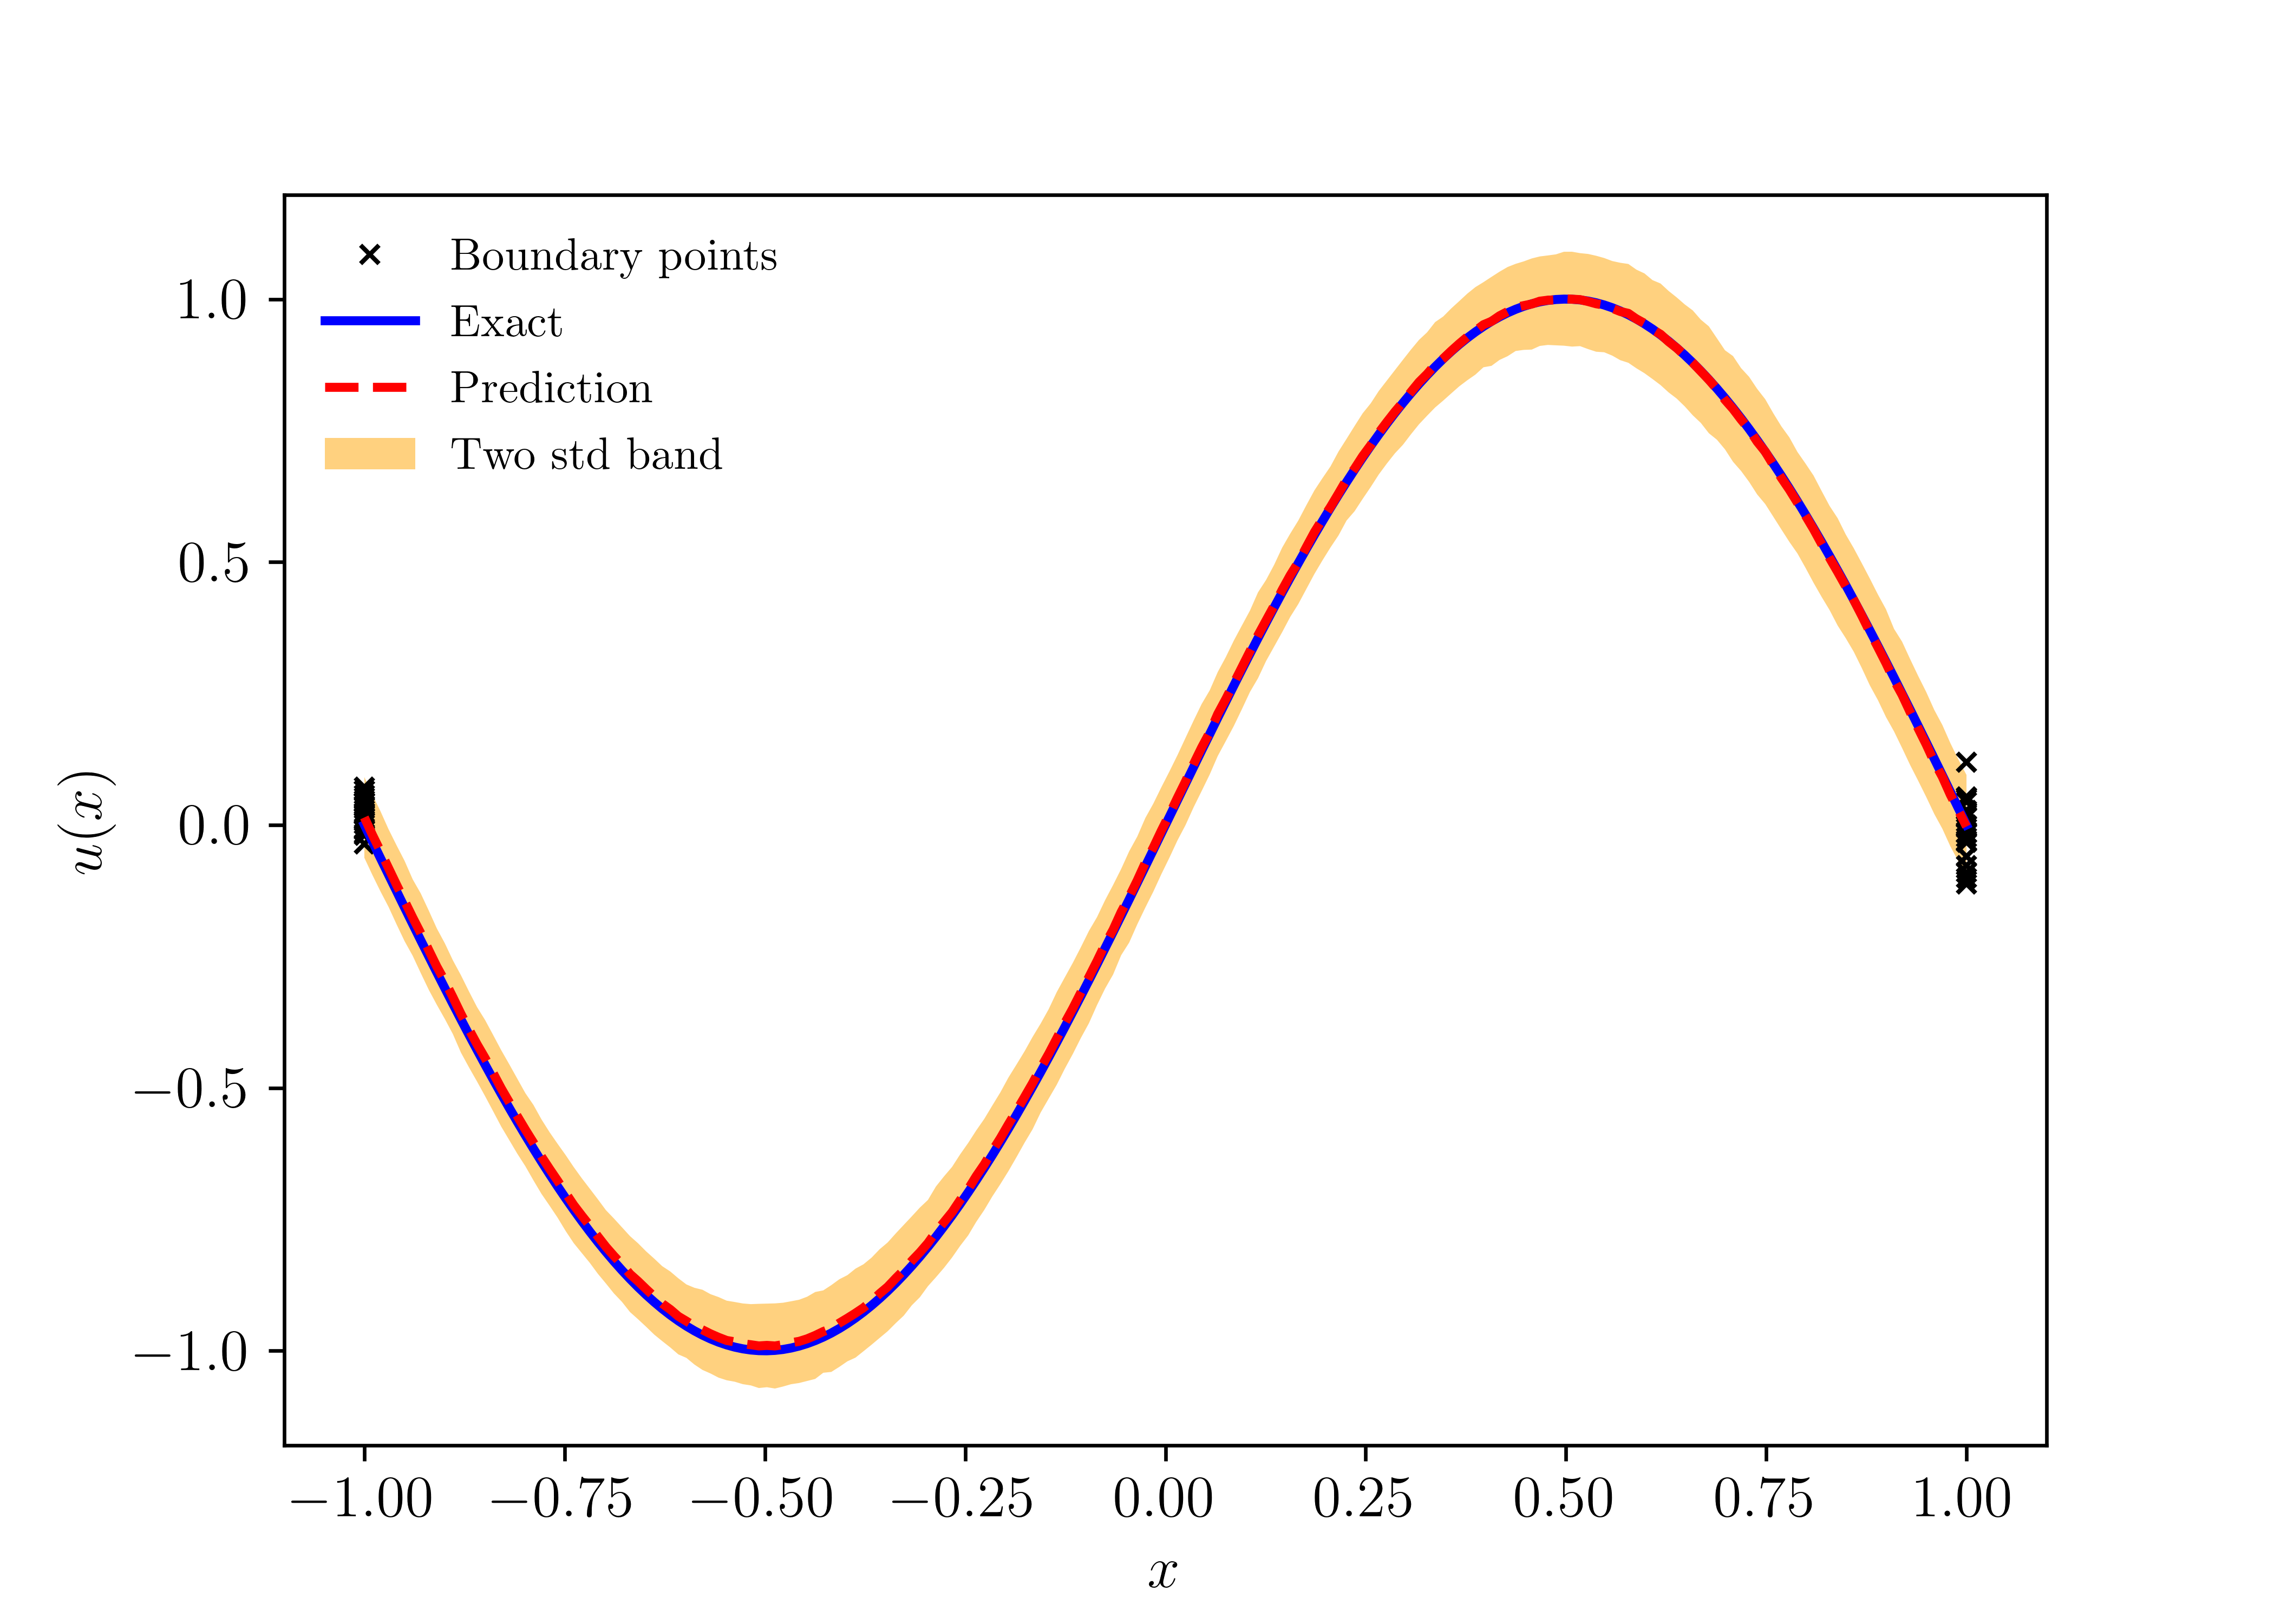
\includegraphics[width=\textwidth]{./ODE_UQPINN/ODEnew1.png}
    \end{minipage}
\end{frame}

\begin{frame}{Burgers Equation}
    \begin{align*}
        \frac{\partial u}{\partial t} &+ u\frac{\partial u}{\partial x} - \nu \frac{\partial^2 u}{\partial x^2} = 0
         \quad &x&\in[-1,1], t\in[0,1]
        \\
        u(0,x) &= -sin(\pi x)
        \\
        u(t, x) &= 0 \quad & x&=\{-1, 1\}
        \\
        \nu &= \frac{0.01}{\pi}
    \end{align*}
\end{frame}



\begin{frame}{Darcy}
    \begin{align*}
        \nabla_{\vec x} &(K(u)\nabla_{\vec x} u(\vec x)) = 0  & \vec x&\in [0,L_1]\times [0,L_2]
        \\
        u(\vec x) &= 0 & x_1 &= L_1
        \\
        -K(u) &\frac{\partial u(\vec x)}{\partial x_1} = q & x_1 &= 0
        \\
        K(u) & = K_s \sqrt{s(u)} \left(1-(1-s(u)^{\frac{1}{m}})^m\right)^2 & x_2 &= \{0, L_2\}
        \\
        s(u) &= \left(1 + \left(\alpha (u_g - u)\right)^{\frac{1}{1-m}}\right)^{-m}
    \end{align*}
\end{frame}




\end{document}